

% Chapter 

\chapter{Empirical Analysis : Insights from Stylized Facts} % Chapter title

\label{ch:empirical} % For referencing the chapter elsewhere, use \autoref{ch:name} 

%----------------------------------------------------------------------------------------


\headercit{Mais ce n'est pas une question d'{\^a}ge, de chiffres et de stats\\ Moi je te parle surtout de rage, de kif et d'espoir}{Youssoupha}{\textit{, Esperance de Vie}}


\bigskip


%  plan : 

%  1) static morphological analysis : requires a formal link between temporal and spatial correlations ?  -- typology etc can already be interesting --


%  2) presentation of BP case study

%  3) base Bien

%  4) Work with Solène



%----------------------------------------------------------------------------------------


As this quote suggests, a purely quantitative view of the world makes no sense without qualitative counterbalancing. More precisely, we argue that the \textit{clich{\'e}} of an opposition between quantitative and qualitative analysis is an illusion. No distinct boundary exists between both. We propose to call quantitative any process involving computation by a Turing machine, whereas the qualitative will be for us the modeling design process and its interpretations. Therefore both are necessarily closely interlaced in any of our approaches. In particular concerning the construction and the validation or refutation of our theory, empirical analysis on real case studies, implying the extraction and qualification of stylized facts, follows that schema.

% articulation with theoretical questions
% articulation with modeling

We propose in this chapter various empirical analysis on different objects at different scales. A first section begins the examination of static spatial correlations between morphological measures of population density and road network measures on Europe at a 500m resolution. Applying last section of the methodological chapter should provide information on typical spatial scales of interaction between these indicators of territory and network and on dynamical correlations between these. These computation furthermore provide empirical measures on which one model will be calibrated. We then describe a roadmap for statistical analysis on dynamical data of interactions for Bassin Parisien in the last fifty years. An other project using Real Estate transaction data for Parisian Metropolitan Region aim at seeking early warning of network breakdowns. We finally describe potential analyses on South African historical data.



%----------------------------------------------------------------------------------------


%%%%%%%%
%  Section : static analysis
%%%%%%%%

\newpage

\section{Static correlations of urban form and network shape}


Spatio-temporal processes implying diffusion or propagation phenomena generally have a specific structure of correlation. In particular, as derived in section~\ref{sec:spatiotempcorrs}, a static computation of correlation between different instances of a system may under certain conditions provide information on dynamical correlations implied.


% justify scale studied here


%%%%%%%%%%%%%%%%%%
\subsection{Morphological Measures of European Population Density}

\subsubsection{Context}

At the macroscopic scale of system of cities, spatialization of the urban system is reasonably captured by cities position, associated with aggregated city variable to represent entirely the system (see e.g. ontologies of Simpop models~\cite{pumain2012multi} or its successor Marius~\cite{cottineau2014evolution}). At the mesoscopic scale at which we aim to capture morphological manifestations of interactions between transportation networks and territories, structure of the territorial system can be specified by more refined indicators for the morphological aspect. 
% biblio spatial structure etc Florent

\subsubsection{Empirical Analysis}

We study systematically morphological indicators for constant size areas covering European Community. The choice of fixed size areas can be questioned regarding definition of a territorial system, that can be otherwise understood as a consistent spatial entity at a given scale and along certain criteria : \emph{Human territories} as defined by Raffestin (op. cit.) or more generally functionally autonomous spaces\footnote{for example, a tentative of definition of a \textit{Parisian} territory would present many facets. From the subjective territory point of view, intra-muros Parisians consider a strict boundary at \textit{Boulevard Periph{\'e}rique}, whereas close and even further suburbs will be seen as Parisians from the Province. The functional territory of \textit{Metropolitain} extends slightly further than the administrative boundary. Governance perimeters are currently mutating with the Metropolitan governance project. Complementary perceptions of the territory can thus be multiplied.}. Here we choose the mesoscopic scale of a metropolitan center ($\simeq$ 50km) for comparability purposes and because greater scale are no more relevant regarding urban form, whereas smaller scales must contain too much noise. 

Data is the European population density grid~\cite{eurostat} and indicators computation is implemented in parallel using \texttt{R} with Fast convolution raster functions. We show in next figures computed values of morphological indicators (see \cite{le2015forme} for a precise formulation of indicators that are Moran index, average distance, entropy and hierarchy).



%%%%%%%%%%%%%%%%%%
\begin{figure}
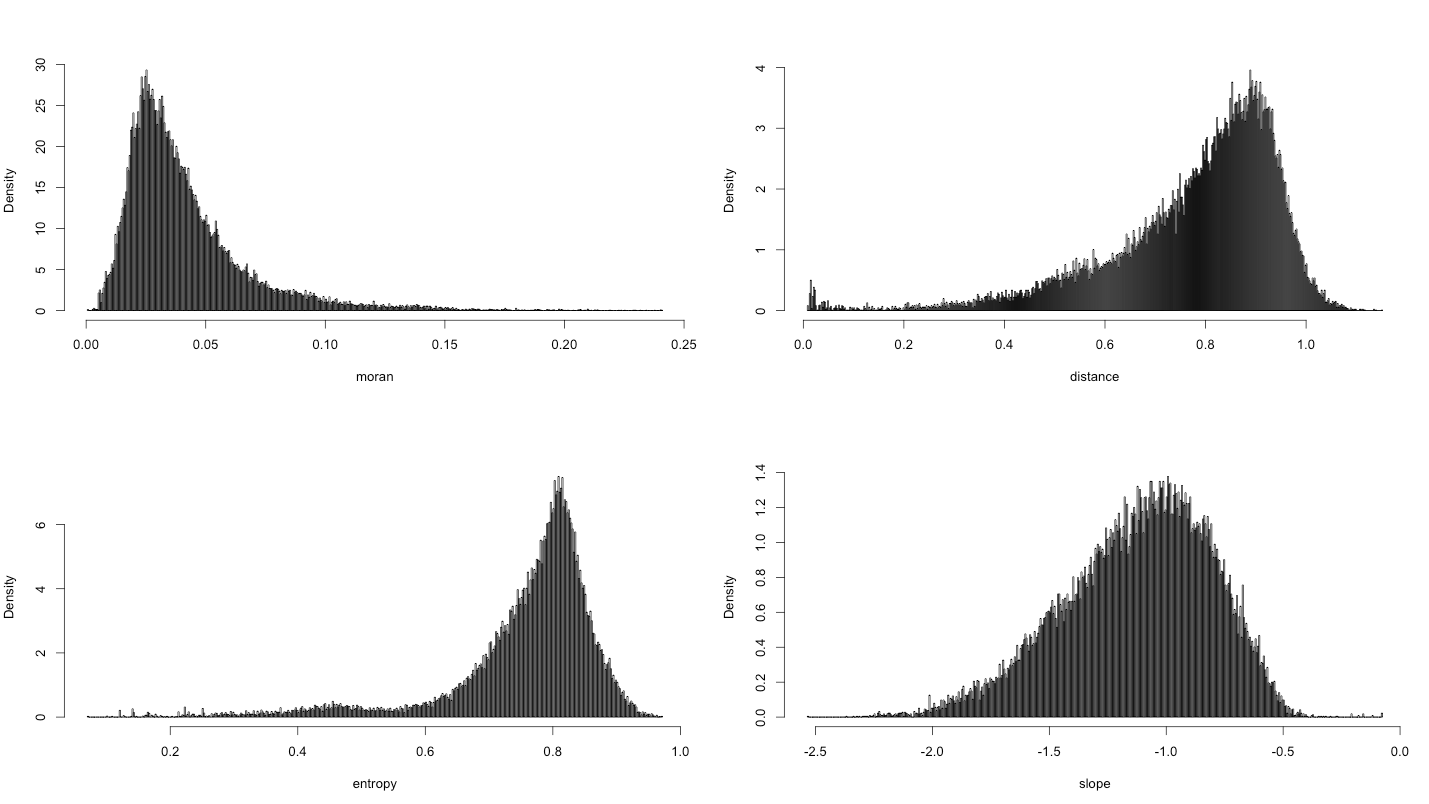
\includegraphics[width=1.2\textwidth]{Figures/PartII/Empirical/Static/Density/hists_GOOD}
\caption[Empirical Distribution of Morphological Indicators]{Empirical Distribution of Morphological Indicators}
\end{figure}
%%%%%%%%%%%%%%%%%%

%%%%%%%%%%%%%%%%%%
\begin{figure}
\hspace{-5cm}
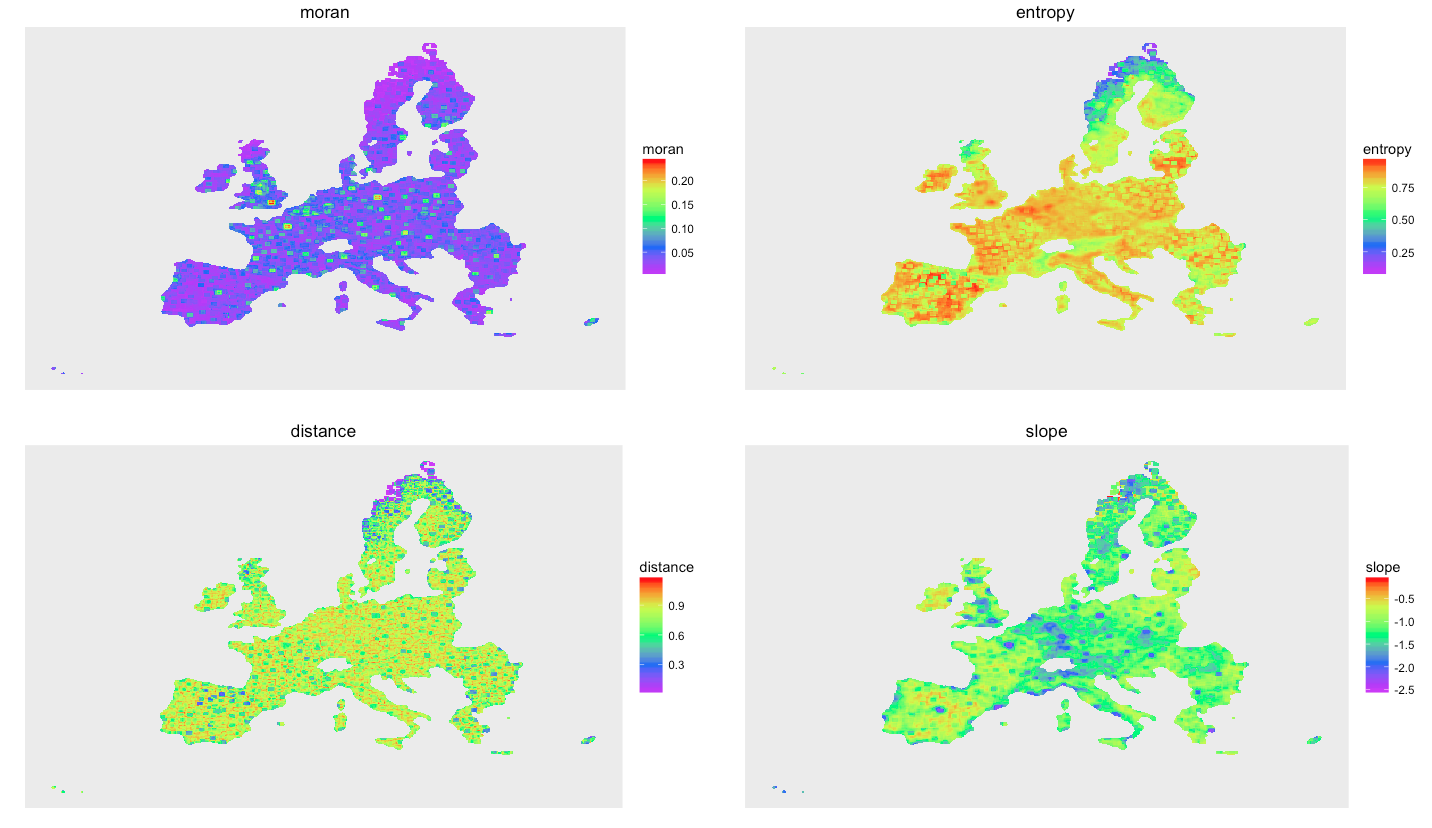
\includegraphics[angle=90,width=1.7\textwidth,height=\textheight]{Figures/PartII/Empirical/Static/Density/all_50km}
\caption[Geographical Distribution of Morphologies]{Geographical Distribution of Morphologies : value of indicators across Europe.}
\end{figure}
%%%%%%%%%%%%%%%%%%


%%%%%%%%%%%%%%%%%%
\begin{figure}
\hspace{-3cm}
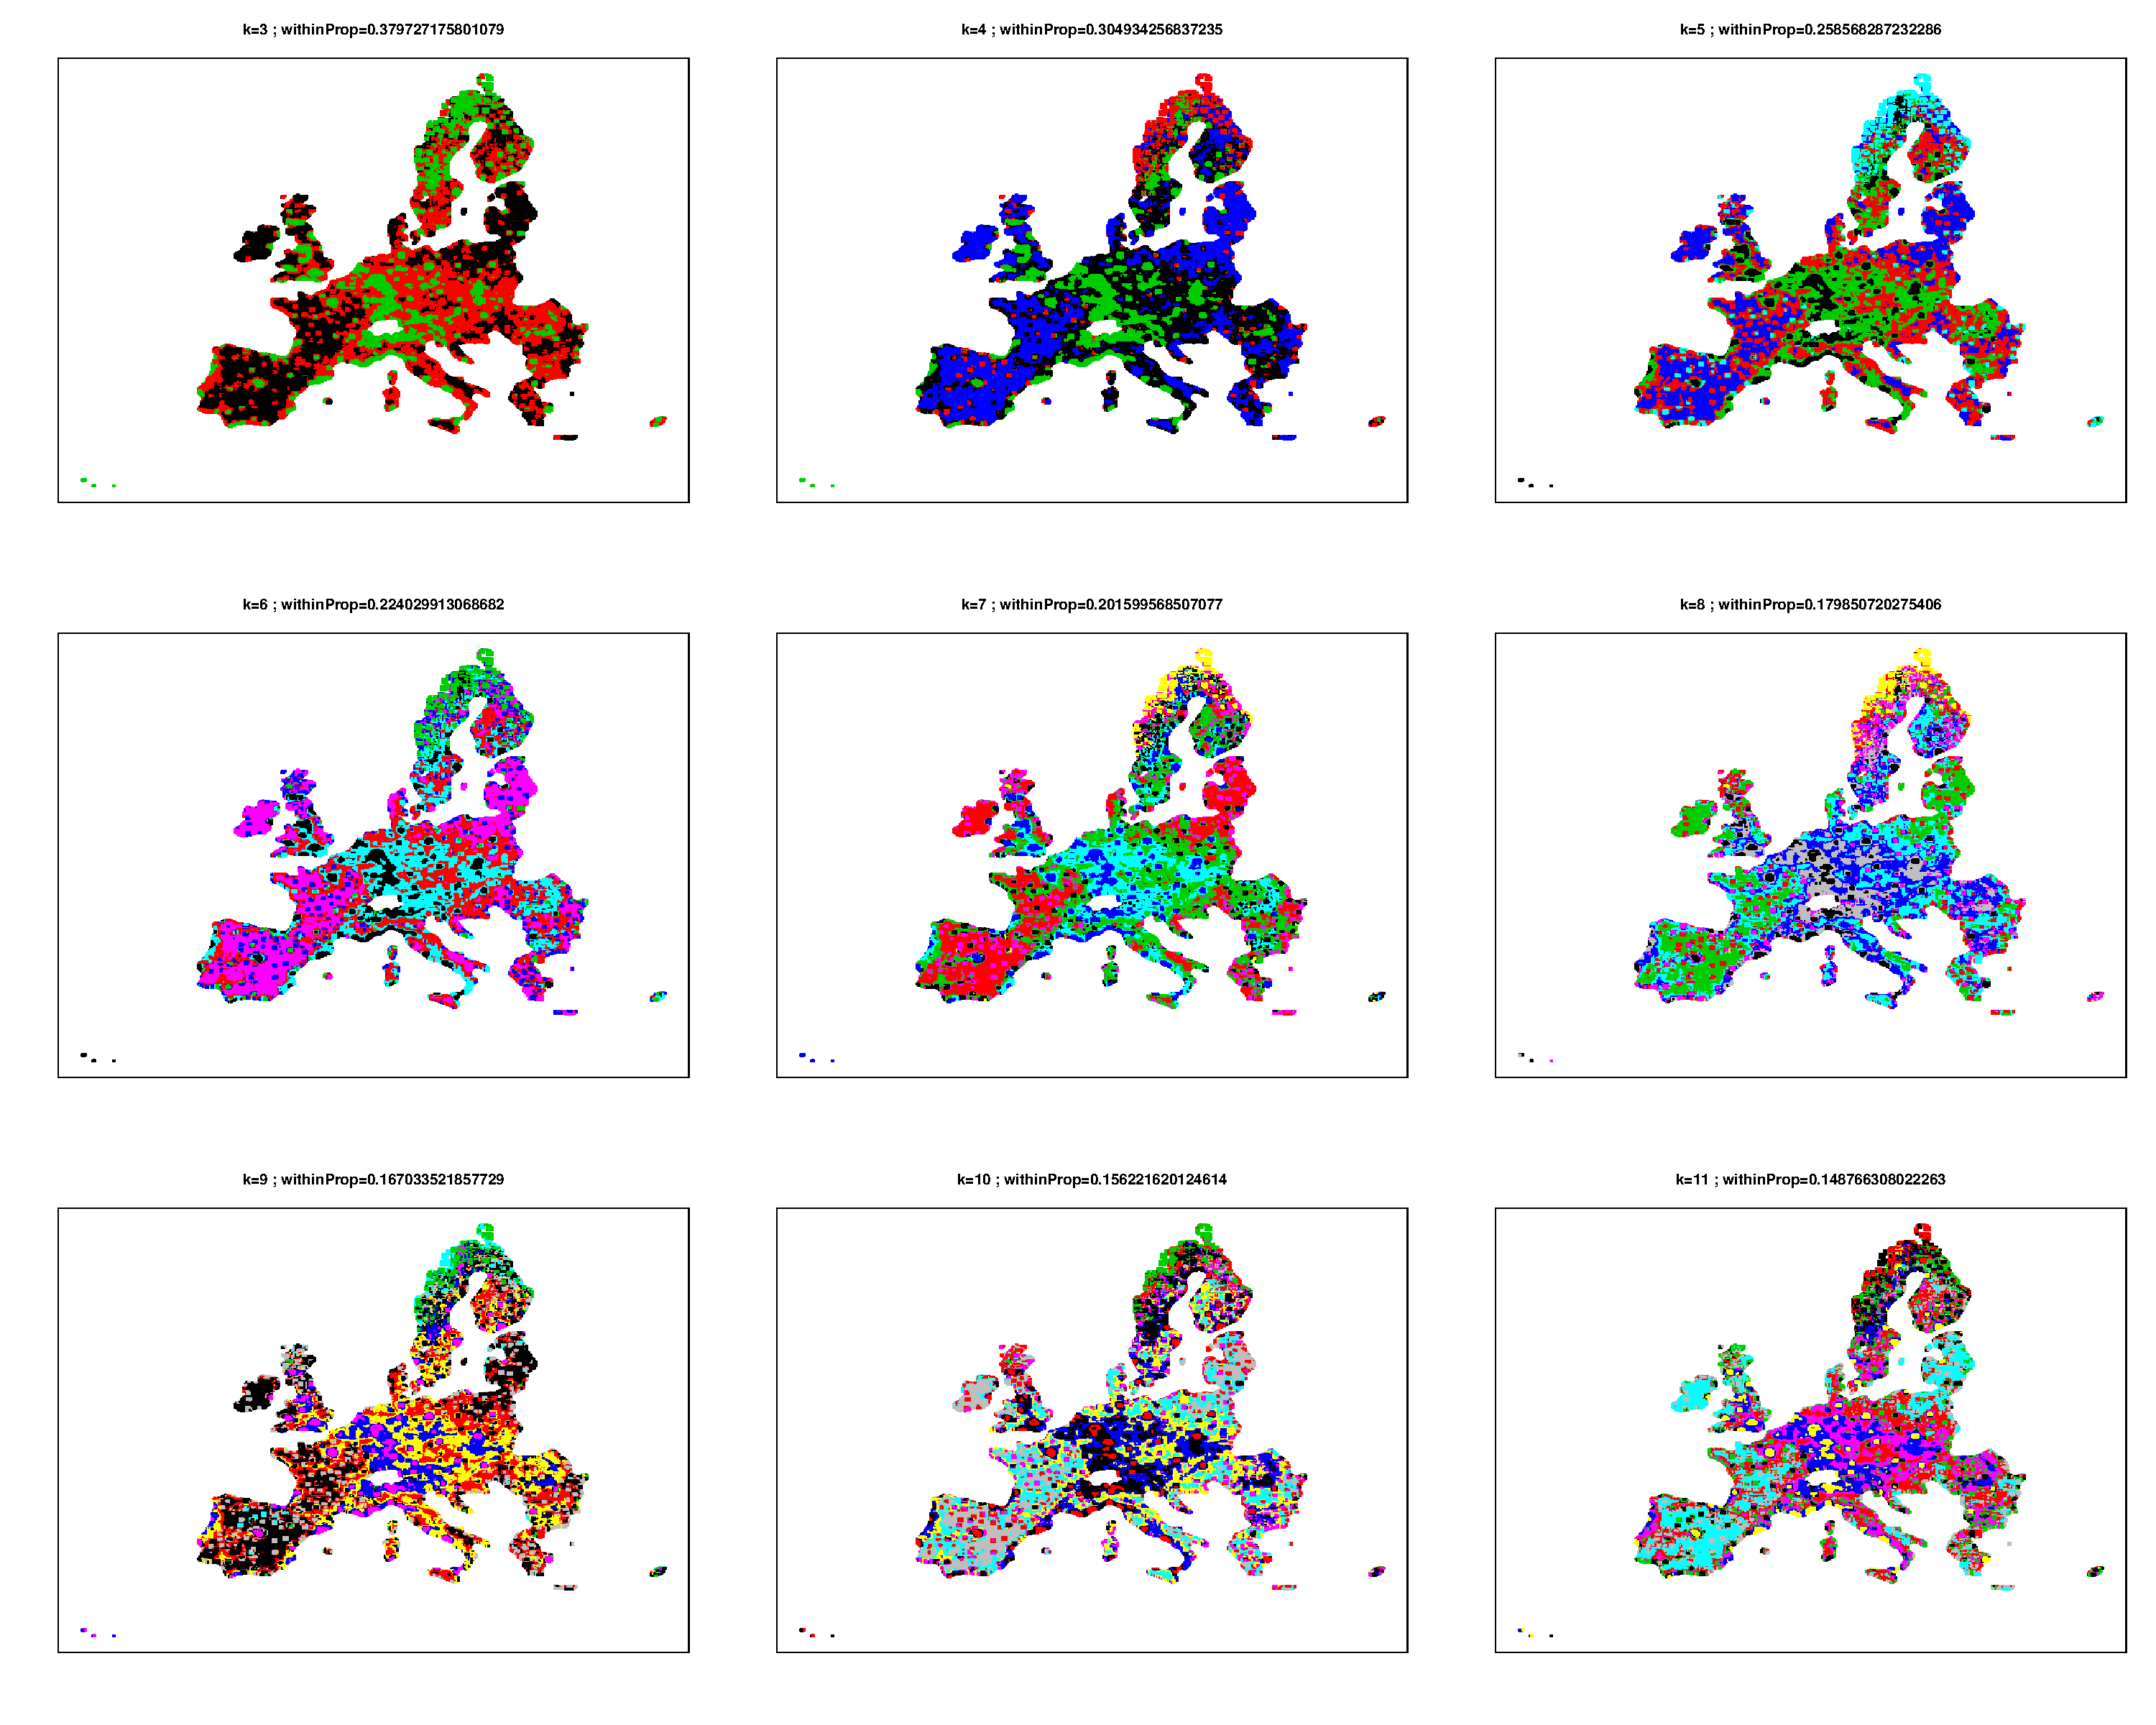
\includegraphics[angle=90,width=1.7\textwidth,height=\textheight]{Figures/PartII/Empirical/Static/Density/clust_k3-11}
\caption[Clustering Analysis of Morphologies]{Clustering Analysis of Morphologies. We present the results of an average k-means for different values of }
\end{figure}
%%%%%%%%%%%%%%%%%%






\subsubsection{Further developments}

In \cite{10.1371/journal.pone.0107042} density grids for other countries across the world (ex. China) are provided\footnote{available at \url{http://www.worldpop.org.uk/}} soo we may repeat our analysis to other regions for comparison purposes.



%%%%%%%%%%%%%%%%%%
\subsection{Network Measures}

We consider network aggregated indicators as a way to characterize transportation network properties on a given territory, the same way morphological indicators yielded information on urban structure. We propose to compute some simple indicators on same extents as for morphology, to be able to explore relations between these static measures. Static network analysis has been extensively documented in the literature, see \cite{louf2014typology} for a cross-sectional study of cities or \cite{2015arXiv151201268L} for exploration of new measures for the road network.


\subsubsection{Data preprocessing}

We work in a first time on road network, which structure is finely conditioned to territorial configuration of population densities. Furthermore, data for present day road network is available through the OpenStreetMap project~\cite{openstreetmap}. Its quality was investigated for different countries such as England~\cite{haklay2010good} and France~\cite{girres2010quality}. It was found to be of a quality equivalent to official surveys for the primary road network.

% data collected from http://download.geofabrik.de/europe.html


\paragraph{Simplification algorithm}

For a given dataset corresponding to a subset of the overall road network, it is necessary to simplify network structure by spatial aggregation as initial data presents very detailed features and thus a very large numbers of nodes ($\simeq 10^10$ for Europe dataset). Such a level of precision is not needed in our study since density data is already aggregated at 500m resolution. It is possible to drastically reduce network size by spatial aggregation of nodes and link replacements. More precisely we use the following procedure :
\begin{itemize}
\item a background raster (which resolution $r$ gives the snapping parameter for aggregation) is constructed from a reference raster and the extent of network. This grid gives spatial aggregation units for network nodes.
\item for each feature of the road dataset, corresponding connected raster cells are stored with corresponding impedance and distance in a sparse adjacency matrix.
\item Network is simplified by iterative suppression of nodes with degree two, with keeping link speed and real length to their effective value.
\end{itemize}


\paragraph{Implementation}

A \texttt{PostGIS} database is used to store raw and simplified network, in order to perform efficient spatial requests, compared for example to initial \texttt{osm} data formats (\texttt{osm} or \texttt{pbf}). However the size of storage of data into this base is much higher (factor 10) so processing was parallelized between european countries. Consistence is ensured by the use of the same common density raster as simplification canvas. Final network is stored into the Postgis database for efficient indicator computation given a spatial extent.


\paragraph{Sensitivity to simplification parameters}

Sensitivity of indicators to raster resolution and to degree simplification algorithm must still be tested to ensure the relevance of data preprocessing.


\subsubsection{Indicators}

Network macroscopic structure is summarized by the following set of indicators, after the simplifications and reductions done in the previous step. Assuming network given by $N=(V,E)$, nodes spatial positions $\vec{x}(V)$ and edges \emph{effective distances} $d(E)$ taking into account impedances and real distances (to include basically network hierarchy), we have indicators :
\begin{itemize}
\item connectivity
\item degree distribution
\item centrality, taken as normalized mean \emph{betweenness-centrality}
\item average path length
\item network diameter
\item mean network speed
\end{itemize}

These indicators are used to capture a rough picture of the structure. Refined work at smaller scales (intra-urban road network) and with more elaborated measures that allow to differentiate more precisely local form, was recently done by Lagesse in~\cite{2015arXiv151201268L}.



\subsubsection{Results}

Computations of network simplification are still ongoing (local parametrization possible only, estimated effective computation time is around 3 weeks). Computations of network indicators and static correlations must then provide the aforementioned insights into interaction processes.


%%%%%%%%%%%%%%%%%%
%\subsection{Effective static correlations}

%%%%%%%%%%%%%%%%%%
%\subsection{Insights for interaction processes}






%----------------------------------------------------------------------------------------


\newpage

\section[Disentangling co-evolutions from causal relations]{Disentangling co-evolutions from causal relations : a case study on \emph{Bassin Parisien}}

Spatial statistics studies on dynamical relations between network and territories are relatively rare. \cite{levinson2008density} does so on London metropolitan area and identifies causalities using lagged variables, but does not disentangle relations in the sense of coupled statistical models that would isolate endogenous effects from coupling effects.

 % study on london with temporal and spatial lag (weird use of spatial statistics) -> expected conclusions but does not really disentangle ?



\subsection{Context Formalization}

%\subsubsection{Variables}

%\paragraph{Description}

We assume a dynamic transportation network $n(\vec{x},t)$ within a dynamic territorial landscape $\vec{T}(\vec{x},t)$, which components are to simplify population $p(\vec{x},t)$ and employments $e(\vec{x},t)$. Data is structured the following way :
\begin{itemize}
\item Observation of territorial variables are discretized in space and in time, i.e. the spatial field $\vec{T}$ is summarized by $\mathbf{T} = \left(\vec{T}(\vec{x}_i,t_j^{(T)})\right)_{i,j}$ with $1\leq i \leq N$ and $1\leq j \leq T$. They concretely correspond to census on administrative units (\emph{communes} in our case) at different dates.
\item Network has a continuous spatial position but is represented by the vector of network distances $\mathbf{N}$
\end{itemize}



%\paragraph{Definitions}



\subsection{On Accessibility}

% accessibility : need to introduce it ?
%  -> read Weibull

The notion of accessibility has been central to regional science since its introduction and systematization in planning around 1970. 

%\paragraph{Existence of accessibility}

%An elegant axiomatic definition is derived in~\cite{weibull1976axiomatic}. Starting from expected properties of an accessibility function $A$ that associate a value to \emph{attraction} $a$ and distance $d$, defined on the set of discrete spatial configurations $\mathcal{C} = \cup_{n\in \mathbb{N}}{(d_i,a_i)_{1\leq i \leq n}}$. These properties include (among technical others with no thematic meaning) :
%\begin{enumerate}
%\item $A$ is invariant regarding the order of the configuration
%\item $A$ decrease with distance at fixed attraction and increase with attraction at fixed distance
%\item $A$ is invariant when adding null attractions and constant configurations
%\end{enumerate}

%A canonical decomposition of any accessibility function 


As already introduced in the first chapter, we question the notion of accessibility : \textit{Is the notion of accessibility crucial for statistical analysis ?}

\medskip


Weibull has proposed an axiomatic approach to accessibility~\cite{weibull1976axiomatic}, deriving a canonical decomposition for any \emph{attraction-accessibility} function $A(a,d)$, assuming expected thematic axioms among others technical ones that are :
\begin{enumerate}
\item $A$ is invariant regarding the order of the configuration
\item $A$ decrease with distance at fixed attraction and increase with attraction at fixed distance
\item $A$ is invariant when adding null attractions and constant configurations
\end{enumerate}
Then $A$ verifies these if and only if it is of the form

\[
A\left[(a_i,d_i)\right] = T\left(\bigoplus_i z(d_i,a_i)\right)
\]

where $T$ is increasing with null origin, $z$ is a \emph{distance substitution function} (i.e. verifying axiom 2) and $\oplus$ a \emph{standard composition} associating two attractions at zero distance to th corresponding unique one. 

It means that well suited matrices of autocorrelation should capture accessibility in regressions ; or it must be captured by non-linear regression on $\mathbf{N}$. It may reveal some kind of intrinsic accessibility that is related to real phenomena (that we expect to fit with calibrated functions of accessibility based on Hedonic models e.g.) Seeing accessibility as a potential field is an equivalent vision : given any stationary dynamic for $n,\vec{T}$, Helmoltz theorem states that it derives from a potential (can be adapted to non-stationary dynamics with a time-varying potential).

%\paragraph{Continuous approach and accessibility potential}

% Paul : Helmoltz-Hodge theorem to infer potential field from speed spatial field ?
%  Q : what are trajectories ? dirac field has no rotational -> continuous approach does not work ?


\subsection{Data}

We will work on a novel dataset provided by \noun{Le Nechet}, that consists in main road infrastructures with their opening dates and train network for network dynamics, and in population and employments of communes at census dates, for Bassin Parisien on the last fifty year. The temporal granularity due to census temporal step may be an obstacle to obtain good dynamical statistics.


\subsection{Statistical Tests}


The following large set of analysis are to be tested (non exhaustive) :
\begin{itemize}
\item On raw data :
\begin{itemize}
\item Multivariate models
\[\mathcal{L}\left[\mathbf{T},\mathbf{N}\right]\sim \varepsilon\]
\item Autocorrelated univariate models
\[(\mathbf{I} - \Sigma R W) \mathbf{X} \sim \varepsilon\]
\item Autocorrelated multivariate models \[(\mathcal{L}' - \Sigma R W)\left[\mathbf{T}+\mathbf{N}\right] \sim \varepsilon\]
\item Geographically Weighted Regression~\cite{brunsdon1998geographically}
\[
\mathcal{L}\left[\mathcal{G}\left(\mathbf{T},\mathbf{N}\right)\right] \sim \varepsilon
\]
\item Granger causality tests : \cite{xie2009streetcars} use for example Granger causality to link transit with land-use changes.
\end{itemize}
\item On data returns :
\begin{itemize}
\item Autoregressive multivariate models
\[\mathcal{L}\left[(\Delta \mathbf{T}(t_{j'}))_{j'\leq j},(\Delta \mathbf{N}(t_{j'}))_{j'\leq j}\right] \sim \varepsilon\]
\item Autoregressive autocorrelated multivariate models : idem with spatial autocorrelation term.
\item Synthetic Instrumental Variables : static territory and/or network ?
\end{itemize}
\end{itemize}



%\subsubsection{Bivariate linear models}

%\subsubsection{Autocorrelated univariate models}

%\subsubsection{Autocorrelated multivariate models}

%\subsubsection{Granger causality tests}

%\cite{xie2009streetcars} use Granger causality to link transit with land-use changes.

%\subsubsection{Autoregressive multivariate models}

%\subsubsection{Autoregressive autocorrelated multivariate models}


\bigskip

\subsection{Expected results}

We expect from these analyses to test at these spatial and temporal scales, and on a particular metropolitan case study, the assumption on network necessity for the territorial system of functional job commutings.






%----------------------------------------------------------------------------------------

\newpage

\section[Real Estate Trajectories]{Early warnings of Network Breakdowns : socio-economic and real estate trajectories}


\subsection{Context}

Various aspects of territories are concerned by interactions with networks. In previous empirical studies, no socio-economic attributes of populations inhabiting the territory nor economic values for land and real estate was considered. Both are however crucial elements of territorial dynamics and are extensively studied in fields such as territorial analysis or urban economics : for example, \cite{homocianu:tel-00359302} studies households residential choices to understand land-use transportation interactions. We propose here to use a database of Real Estate transactions for Parisian region on the last 20 years, with 2 years temporal granularity and exact spatial coordinates. \cite{guerois2009dynamique} used it to make typologies of spatial dynamics of Parisian real estate. This project is conjointly done with \noun{Le Corre} whose strong thematic knowledge on Real Estate financial properties will bring insight for spatial typologies of temporal trajectories.% results using base bien.



\subsection{Preliminary Results}

We show in Fig.~\ref{fig:realestate} typologies of temporal transactional profiles for total stocks. Temporal dynamics show different reactions of local territories to the 2008 crisis, in particular a strong differentiation between urban and rural areas. More precise classification into urban territories are still to be investigated when the analysis will be pushed further.



%%%%%%%%%%%%%%%
\begin{figure}
\hspace{-3cm}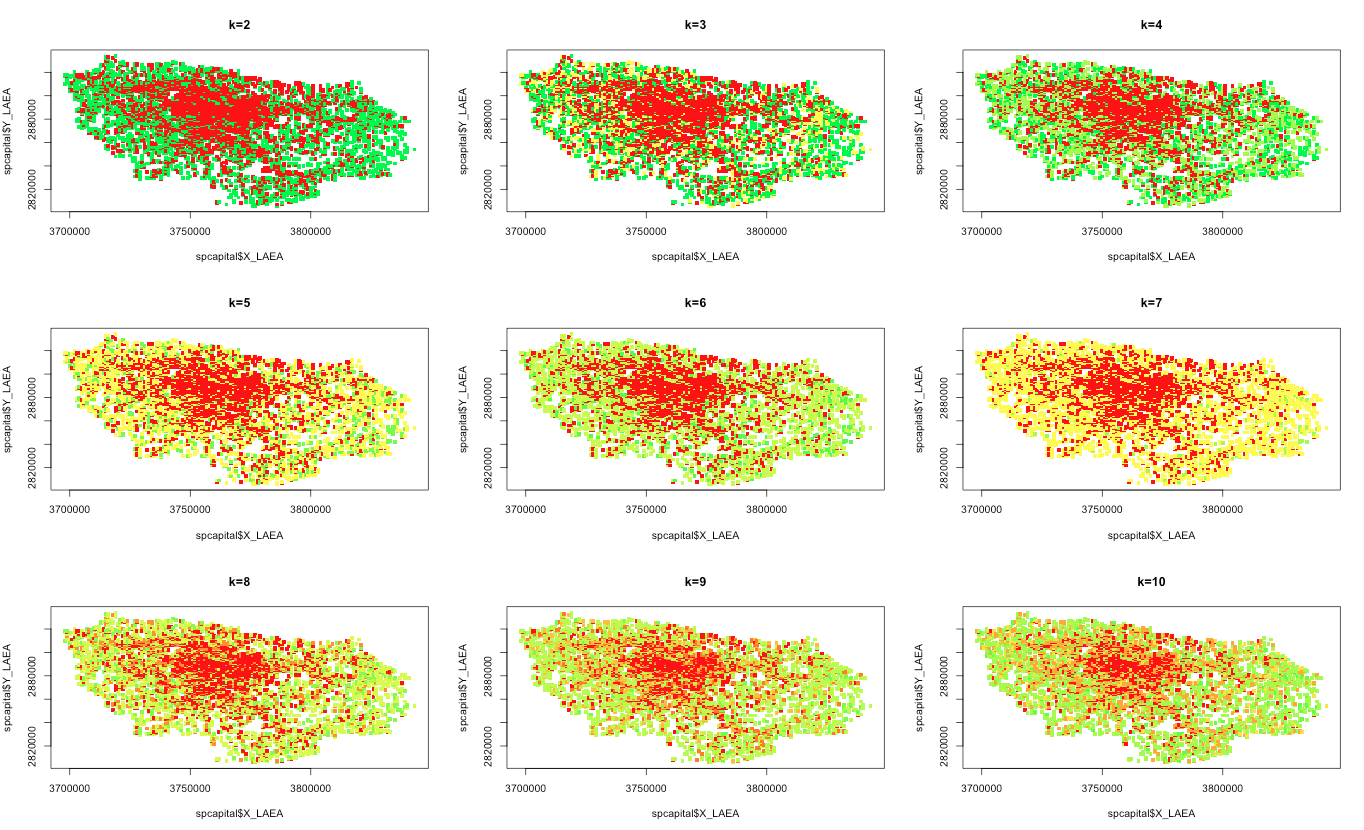
\includegraphics[width=1.4\textwidth]{Figures/PartII/Empirical/RealEstate/normalized_k2-10}
\smallskip
\hspace{-3cm}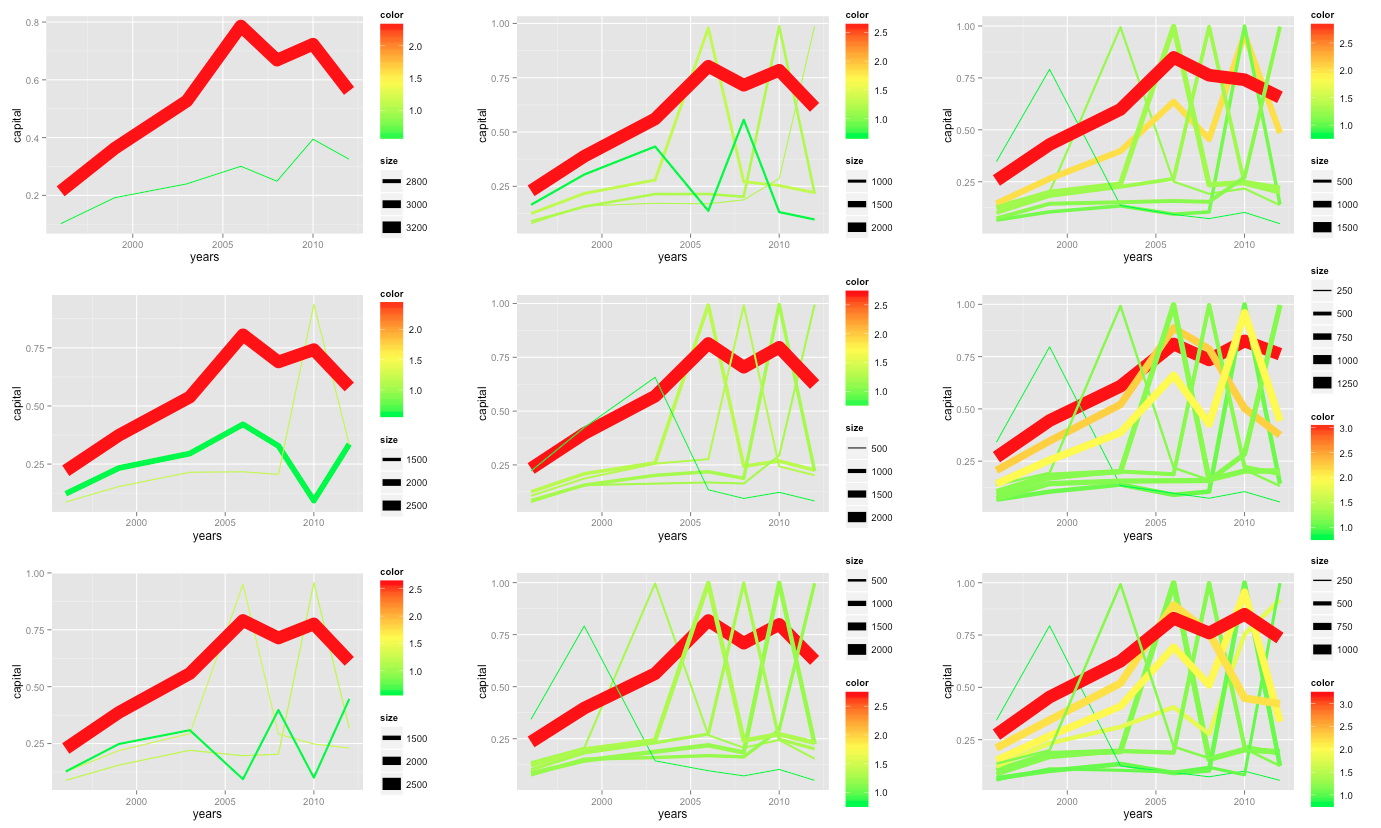
\includegraphics[width=1.4\textwidth]{Figures/PartII/Empirical/RealEstate/trajectories_normalized_k=2-10}
\caption[Typology of Real Estate trajectories]{Typology of Real Estate trajectories. Locations were categorized using averaged k-means on time-series. We show maps and time series for value of k from 2 to 10.}
\label{fig:realestate}
\end{figure}
%%%%%%%%%%%%%%%



\subsection{A strategy to investigate early warnings of network breakdowns}


The span of the end of this database coincides with planification phases of the Grand Paris Express that we already mentioned. We aim to seek for early warnings of potential station implantation, in correspondance with different stages of the project, in order to verify if intrinsic territorial dynamics were already present or if the announcement of a new station induced a local phase transition.





%----------------------------------------------------------------------------------------

\newpage

\section[South-African historical events as instruments]{South-African historical events as instruments to understand network-territory relations}

\subsection{Context}

The method of instruments in statistics~\cite{angrist1996identification} is used to identify causal relationships between variables, in a different way than Granger causality test for example. Trying to identify causalities between network dynamics and territorial dynamics is of crucial importance to test our theoretical assumption on the existence of co-evolution.

A project planned in collaboration with \noun{Baffi}, based on her thesis project~\cite{baffi2016thesis} that studied qualitatively the role of South African railways in segregations and integration processes, aims to use an extensive database of railway growth and population dynamics in cities on the last 100 years produced during the thesis. In particular, she showed qualitatively that dynamics between territories and networks profoundly changed at the end of the apartheid, transforming a tool of sordid planned segregation (network shaped was optimized to minimize unwanted accessibility) into an integration tool thanks to recent changes in network topology patterns.

\subsection{Objectives}

We can use first the particular shape of that network to control on local and global topology effects (but this is quite equivalent as controlling on accessibility), and in a second time the historical events as statistic instruments, assuming that territorial dynamics and network dynamics responded differently to these. We expect to learn from these project informations on interactions at long time scale and large spatial scale, in a very particular context of constrained growth.







